\chapter{Entwicklungsumgebung}
\label{chap:entwicklungsumgebung} Da bereits 3D Slicer als Framework feststeht,
ist keine weitere Forschung nötig, um die richtige Programmiersprache auszuwählen.
Jedoch gibt es eine kleine Auswahl zu treffen. 3D Slicer unterscheidet zwischen zwei
Arten von Modulen, die \ac{CLI} Module, welche in der Sprache C++ geschrieben
werden und die Scripted Moduls, die eine Python Implementierung verlangen. Da
die anatomische Segmentierung ohnehin in einem IPython-Notebook bereitliegt, fiel
die Wahl hier auf die Scripted Moduls. So kann auch die breite Palette der
Python-Pakete genutzte werden. Um den Entwicklungsprozess etwas zu vereinfachen,
wurde während der Entwicklung auf ein Modul von Slicer zurückgegriffen, das speziell
für Entwickler entworfen wurde. Die Abbildung \ref{fig:entwicklungsumgebung}
verdeutlicht dieses Tool.

\begin{figure}[h]
	\centering
	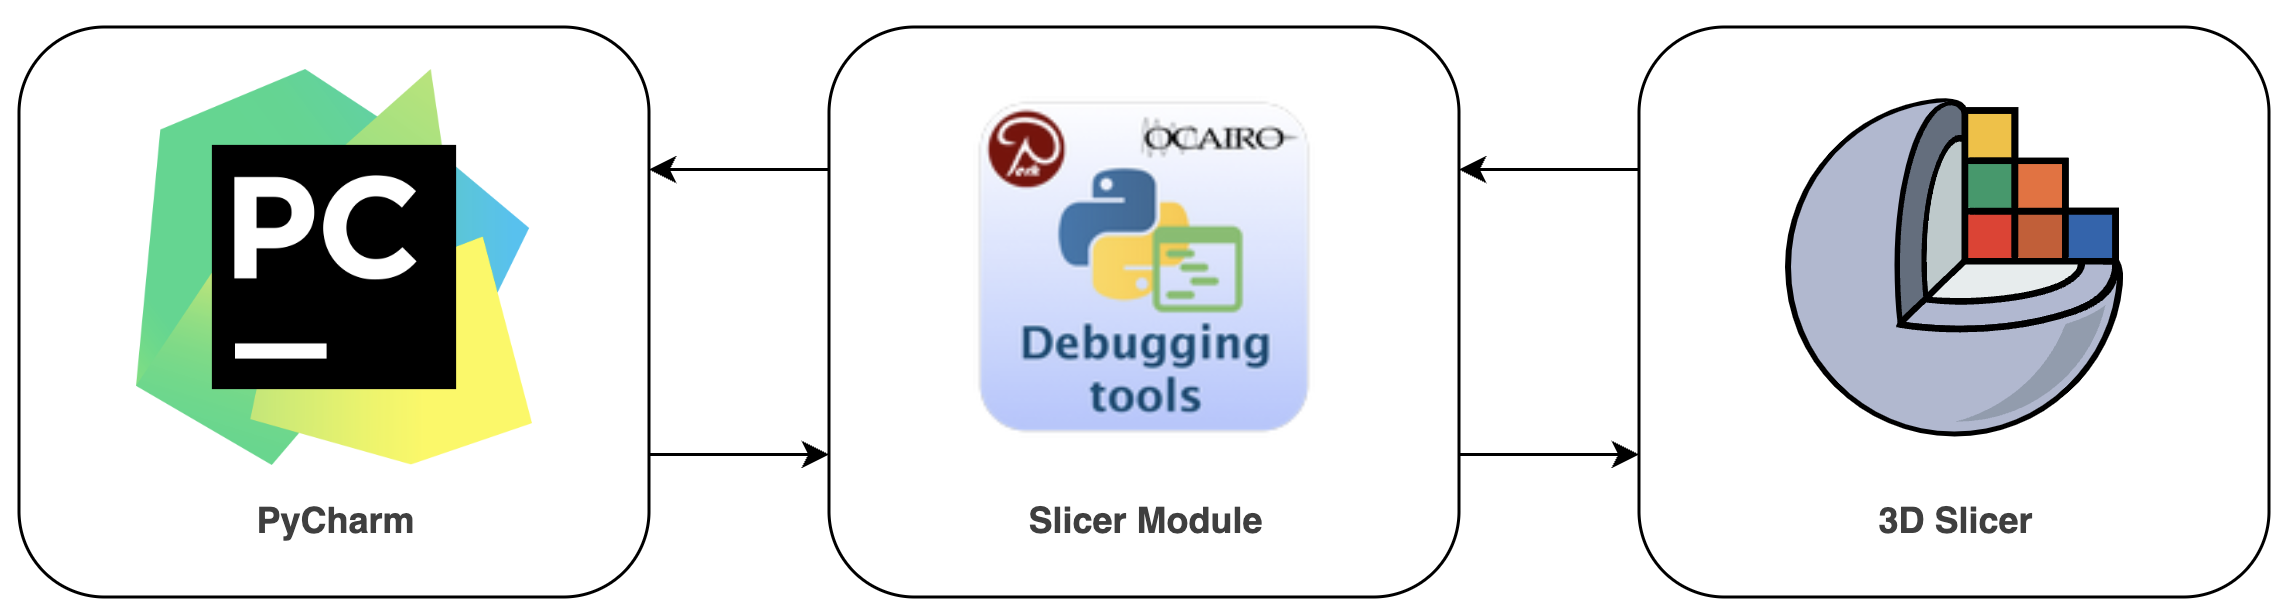
\includegraphics[width=0.6\textwidth]{img/Entwicklungsumgebung.png}
	\caption{Umgebung während der Entwicklung mit 3D Slicer und PyCharm}
	\label{fig:entwicklungsumgebung}
\end{figure}

Mit dem Debugging Tool lässt sich eine gewohnte Umgebung reproduzieren, in der
der Quellcode Schritt für Schritt analysiert werden kann \citep[vgl.][]{slicerdebuggingtools}.
Speziell bei der Fehlersuche ist dieses Tool eine sehr gute Unterstützung. Die Abbildung
beschreibt weiter, das als Umgebung für das Erstellen des Programmcodes die
Software Pycharm verwendet wird. Pycharm ist eine Lösung der Firma Jetbrains,
für das Erstellen von Python-Quellcode. Dieses Tool bietet eine breite Palette an
Funktionalitäten, die das Erstellen von Software vereinfachen und als \textit{State
of the Art} bezeichnet werden kann \citep[vgl.][]{jetbrains2024}.

Für die Interaktion mit der Slicer Kernanwendung stellt der Python-Interpreter
das Paket \texttt{slicer} zur Verfügung. Hierdurch lassen sich diverse
Mechanismen steuern. Wichtig ist hierbei, dass das Paket \texttt{slicer} nicht auf
\ac{PyPi} zu finden ist. Es ist nur in der Python-Umgebung vorhanden, die mit
der Slicer Installation einhergeht. Neben dem Paket \texttt{slicer} sind noch
viele weitere Pakete verfügbar, die sich in der medizinischen Bildbearbeitung durchgesetzt
haben. Für eine komplette Auflistung aller Python-Pakete sei an dieser Stelle
auf die Dokumentation von Slicer verwiesen \citep[vgl.][]{slicer2024}.

Auch die Versionierung des Quellcodes wurde von Anfang an in den Entwicklungsprozess
integriert. Da die Software ohnehin über ein öffentliches GitHub-Repository in
Slicer eingebunden wird, diente dieses zugleich als zentrales Werkzeug zur Versionskontrolle.
Im Hintergrund kommt dabei selbstverständlich Git zum Einsatz. Der Link zum öffentlichen
Repository kann dem Anhang entnommen werden.

Damit während der Entwicklung auch Teilbereiche der Software bereits getestet werden
können, werden Testdaten benötigt. Bei diesen Testdaten handelt es sich um originale
Mikro-\ac{CT}-Aufnahmen im Format \ac{16Int}, \ac{ISQ}. Diese wurden auf einem
Server an der \ac{LMU} in München bereitgestellt. Der Zugriff auf den Server
erfolgt über den \textit{x2goclient}. Heruntergeladen wurden die Daten über eine
\ac{SSH} Verbindung. Bei den Mikro-\ac{CT}-Bildern handelt es sich ausschließlich
um Aufnahmen der Zahnkrone. Mit dem Zugriff auf den Server an der \ac{LMU} konnten
auch diverse Pythonumgebungen zum Verarbeiten von Daten genutzt werden. Dies war
in erster Linie für ein Nachvollziehen und Verstehen der anatomischen
Segmentierung hilfreich.

Neben der eigentlichen Umgebung von Slicer und den Entwicklerwerkzeugen steht
zur Entwicklung auch ein Python Paket zur Verfügung, das von Herrn Prof. Rösch
speziell für die Klinik an der \ac{LMU} erstellt wurde. Dieses Tool beinhaltet
diverse Funktionalität für das Verarbeiten von medizinischen Bilddaten. Speziell
für die Mikro-\ac{CT}-Aufnahmen der Klinik.

Nachdem die Entwicklungsumgebung definiert und eingerichtet wurde, kann nun auf die
konkrete Methodik eingegangen werden, die zur Umsetzung dieser Schnittstelle
verwendet wird. Dabei werden sowohl die Anforderungen an die Erweiterung beschrieben,
als auch die konzeptionellen Überlegungen.

% ---------------------------------------------------------------------------------------